\chapter{Experimental Setup}
\label{chap:experimental_setup}
This chapter describes the experimental setup, introducing the datasets employed to evaluate the proposed method, followed by an outline of a distinct \emph{Configuration} setup, which encompasses the selection and rationale behind all parameters. Subsequently, the \emph{Preprocessing} steps are discussed, along with specific settings related to \emph{Training}, \emph{Validation}, and \emph{Testing}. The \emph{Monitoring} subsection enumerates the metrics utilized for this project and elaborates on additional techniques such as learning curves, \ac{wandb} (Weights and Biases), early stopping, and the ablation setup, which measures similarity across different subsets used for training.

The setup is designed to comprehensively assess the method's performance, scalability, and robustness. It is based on the model production cycle presented in \secref{subsec:segmentation_framework}, which systematically creates, trains, and evaluates new models using a specified configuration.

\section{Datasets}
\label{sec:datasets}
Three datasets were used to evaluate the proposed methodology's performance. These include the \acf{MFD} \cite{10.1371/journal.pone.0263656}, the \acf{SLD} from \ac{ISIC} \cite{DBLP:journals/corr/abs-1710-05006} and the \acf{IDRID} \cite{h25w9818} where each of them presents unique challenges and properties which allows for a comprehensive analysis of the proposed approach.

\textbf{\emph{The Medaka Fish Dataset}} consists of images of the Medakas fish cardiac system. The dataset contains four classes, including the background class. The images display varying complexity, as they contain multiple cellular structures and patterns. The Bulbus class, illustrated as the purple mask in \figref{dataset_labels} on the image (d), is the hardest class to predict as the cardiac outflow is not as clearly delineated as the Atrium and Ventricle \cite{10.1371/journal.pone.0263656}.

\textbf{\emph{The Skin Lesion Dataset}} contains dermoscopic images of skin lesions, including various types of skin cancer, such as melanoma, basal cell carcinoma, and squamous cell carcinoma. The dataset also contains benign skin lesions, such as nevi and seborrheic keratoses. This dataset aims to accurately delineate the borders of skin lesions, which is an essential part of the diagnosis and treatment planning for skin cancer \cite{DBLP:journals/corr/abs-1710-05006}.

\textbf{\emph{The Indian Diabetic Retinopathy Image Dataset}} contains high-resolution retinal images from patients with diabetic retinopathy, a diabetes-related complication and leading cause of vision loss worldwide \cite{STITT2016156}. The dataset features images exhibiting varying degrees of diabetic retinopathy severity alongside standard retinal images for comparison. The primary objective of this dataset is to identify and classify different retinal lesions, such as microaneurysms, hemorrhages, and exudates, which can offer valuable insights for the early detection and treatment of diabetic retinopathy. Due to its highly imbalanced properties and distribution of lesions across the entire retina, this dataset presents significant challenges for prediction tasks.

\begin{figure}[H]%[htbp]
  \centering
  \subfigure[]{\includegraphics[width=\imgWidthThree]{images/medaka.png}}
  \subfigure[]{\includegraphics[width=\imgWidthThree]{images/skin_lesion.jpg}}
  \subfigure[]{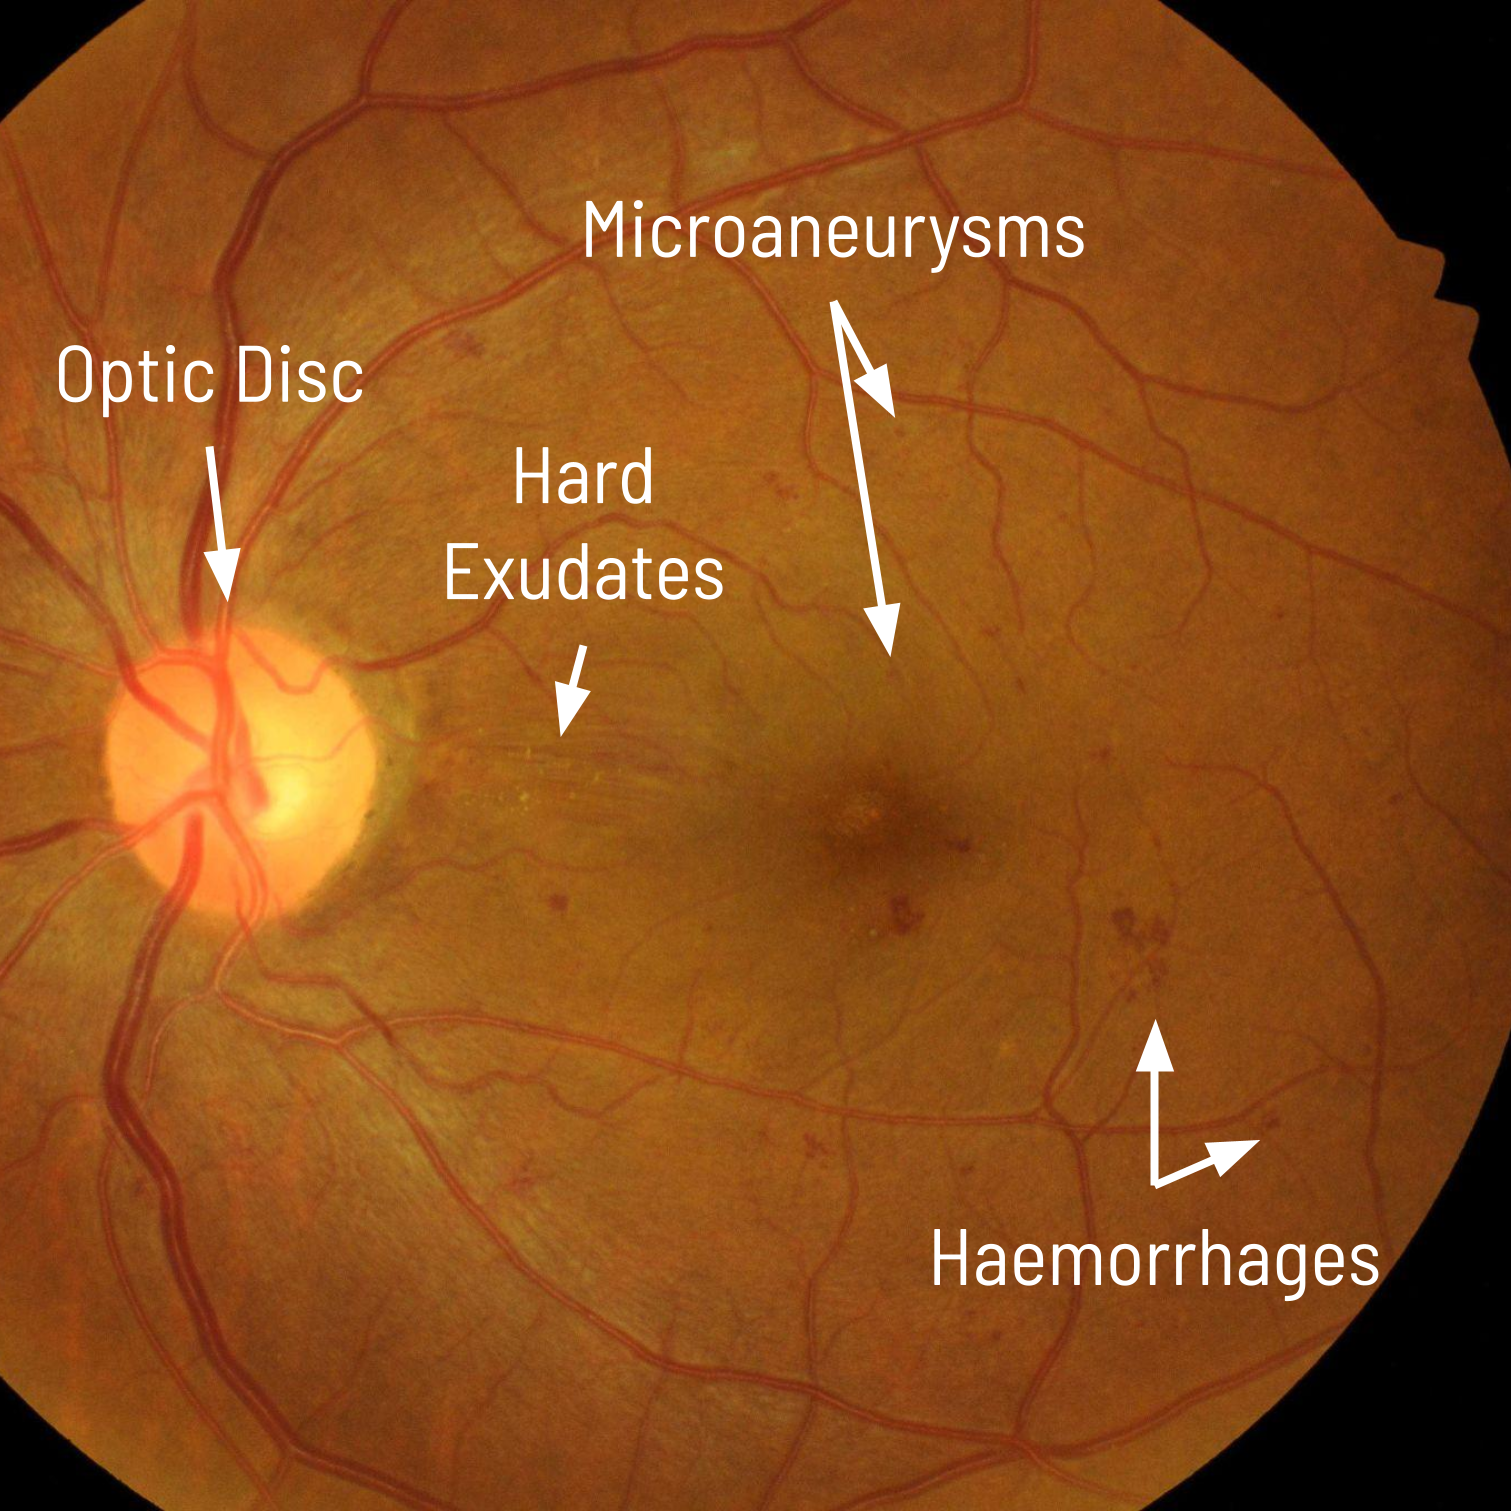
\includegraphics[width=\imgWidthThree]{images/IDRID_sample.png}}
  \subfigure[]{\includegraphics[width=\imgWidthThree]{images/00020_mask.png}}
  \subfigure[]{\includegraphics[width=\imgWidthThree]{images/ISIC_0000007_mask.png}}
  \subfigure[]{\includegraphics[width=\imgWidthThree]{images/IDRID_mask.png}}
  \caption[Dataset samples and output label]{Labels and masks of three different datasets used to evaluate this project. The image (a) is a label extracted from the \acf{MFD} covering the central vascular system (Bulbus, Atrium, and Ventricle) \cite{10.1371/journal.pone.0263656}. Image (b) displays a sample used along the \acf{ISIC} challenge 2017 \cite{DBLP:journals/corr/abs-1710-05006}, which displays a skin cancer lesion. Image (c) illustrates a sample from the \acf{IDRID}\cite{h25w9818} containing five classes, including the background. The second row (d-f) depicts the corresponding masks from the labels above.}
  \label{dataset_labels}
\end{figure}
\begin{table}[H]
  \resizebox{\columnwidth}{!}{%
    \begin{tabular}{lc|cc|clc}
      \cline{3-4}
                                                                                       &
      \multicolumn{1}{l|}{}                                                            &
      \multicolumn{2}{c|}{\cellcolor[HTML]{000000}{\color[HTML]{FFFFFF} No. images}}   &
      \multicolumn{1}{l}{}                                                             &
                                                                                       &
      \multicolumn{1}{l}{}                                                               \\ \hline
      \rowcolor[HTML]{6638B6}
      \multicolumn{1}{|l|}{\cellcolor[HTML]{6638B6}{\color[HTML]{FFFFFF} Name}}        &
      {\color[HTML]{FFFFFF} Reference}                                                 &
      \multicolumn{1}{c|}{\cellcolor[HTML]{6638B6}{\color[HTML]{FFFFFF} Training}}     &
      {\color[HTML]{FFFFFF} Testing}                                                   &
      \multicolumn{1}{c|}{\cellcolor[HTML]{6638B6}{\color[HTML]{FFFFFF} No. classes}}  &
      \multicolumn{1}{c|}{\cellcolor[HTML]{6638B6}{\color[HTML]{FFFFFF} Distribution}} &
      \multicolumn{1}{c|}{\cellcolor[HTML]{6638B6}{\color[HTML]{FFFFFF} Preprocessing}}  \\ \hline
      \multicolumn{1}{|l|}{Medaka Fish}                                                &
      \cite{10.1371/journal.pone.0263656}                                              &
      \multicolumn{1}{c|}{565}                                                         &
      165                                                                              &
      \multicolumn{1}{c|}{4}                                                           &
      \multicolumn{1}{l|}{94.2\%, 1.8\%, 1.5\%, 2.6\%}                                 &
      \multicolumn{1}{c|}{resize,split,shuffle}                                          \\ \hline
      \multicolumn{1}{|l|}{Skin Lesion (ISIC)}                                         &
      \cite{DBLP:journals/corr/abs-1710-05006}                                         &
      \multicolumn{1}{c|}{2000}                                                        &
      600                                                                              &
      \multicolumn{1}{c|}{2}                                                           &
      \multicolumn{1}{l|}{76.7\%, 23.3\%}                                              &
      \multicolumn{1}{c|}{resize,split,shuffle}                                          \\ \hline
      \multicolumn{1}{|l|}{IDRID}                                                      &
      \cite{h25w9818}                                                                  &
      \multicolumn{1}{c|}{54}                                                          &
      27                                                                               &
      \multicolumn{1}{c|}{5}                                                           &
      \multicolumn{1}{l|}{96.2\%, 1.0\%, 0.95\%, 0.1\%, 1.8\%}                         &
      \multicolumn{1}{c|}{resize,split,shuffle}                                          \\ \hline
    \end{tabular}%
  }
  \caption[Dataset list]{List of three datasets used to evaluate this project. The first entry of the \emph{class distribution} column represents the background class. It can be seen that the datasets, especially Medaka and \ac{IDRID}, are extremely unbalanced. The distribution for the \ac{MFD} corresponds to the classes Background, \textbf{\textcolor{rwuvioletlight}{Bulbus}}, \textbf{\textcolor{rwucyan40}{Atrium}}, and \textbf{\textcolor{rwucyan}{Ventricle}}. For the \ac{SLD} with two classes, it is the Background and the Foreground, and for the \ac{IDRID}, it would be Background, \textbf{\textcolor{rwucyan40}{Haemorrhages}}, \textbf{\textcolor{hardexudates}{Hard Exudates}}, \textbf{\textcolor{microaneurysms}{Microaneurysms}}, and \textbf{\textcolor{rwuviolet}{Optic Disc}}.}\label{tab:datasets}
\end{table}
Table \ref{tab:datasets} offers additional details on the datasets utilized in this project, including their respective sizes, the number of classes, and the corresponding distribution of each class.

\section{Configuration}
\label{sec:configuration}
This section briefly discusses the configuration as the first step of the model production cycle illustrated in \figref{model_production_cycle}. For a more detailed description and the rationale concerning the parameter selection, please refer to \chapref{chap:configuration_details} in the appendices.
\subsection{Parameter Definition}
The configuration involves multiple parameters, categorized according to the framework component they affect. These parameters are divided into two classes: one that maintains a default value throughout the project and another with values that change during training. The changing parameters are further classified into discrete and continuous sets. It is crucial to clearly define these parameters to ensure a consistent and reproducible experimental setup, making it easier to understand the impact of each parameter on the model's performance. The appendix thoroughly analyzes these parameters, specifically in \secref{sec:parameter_definition}. This comprehensive examination allows for a deeper understanding of the parameter space and its influence on the overall results. Based on the parameter analysis, a final predefined sweep configuration \footnote{Sweep configurations are a feature provided by \ac{wandb} which enables different types of hyperparameter exploration including custom-designed training setups.} is established, facilitating a proper and precise evaluation of the model's performance under various conditions.

\subsection{Final Setup}
The final setup for this project encompasses five distinct configurations for each dataset. The first configuration establishes a baseline by training models using the six loss functions described earlier. The second configuration employs a custom approach, systematically iterating through all possible combinations of parameter values. This is feasible because the entire set of parameters originates from a discrete space. The third and fourth configurations utilize an adaptive resource allocation algorithm called Hyperband \cite{DBLP:journals/corr/LiJDRT16}, specifically designed to efficiently identify optimal hyperparameters within a continuous space. It is important to note that the parameter \texttt{selection\_percentage} is set to $1.0$ for the \ac{IDRID} dataset, as using a subset of an already tiny dataset did not seem plausible. The fifth configuration represents a particularly promising combination, which is determined based on the results of previous configurations. Its purpose is to reaffirm the outcomes through a series of repeated trainings. This approach is designed to enhance the stability and reliability of the proposed implementation.

The following table summarizes the presented configurations along their most important parameters for each dataset, resulting in 15 sweep configurations.

% Please add the following required packages to your document preamble:
% \usepackage{graphicx}
% \usepackage[table,xcdraw]{xcolor}
% If you use beamer only pass "xcolor=table" option, i.e. \documentclass[xcolor=table]{beamer}
\begin{table}[H]
  \centering
  \resizebox{\textwidth}{!} &
    {\color[HTML]{FFFFFF} Strategies} &
    {\color[HTML]{FFFFFF} Dataset} &
    {\color[HTML]{FFFFFF} Time based} &
    {\color[HTML]{FFFFFF} Epoch} &
    {\color[HTML]{FFFFFF} Model} &
    {\color[HTML]{FFFFFF} Config type} &
    {\color[HTML]{FFFFFF} Model count} &
    {\color[HTML]{FFFFFF} Auto LR} &
    {\color[HTML]{FFFFFF} Img size} \\ \hline
  1  & single         & 0.32,0.64,1.00 & -                           & Medaka      & False & 100 & UNET & Baseline   & 18  & False & 256 x 256 \\ \hline
  2  & double,triple  & 0.32,0.64,1.00 & MAX,MIN,AVG,HARMONIC,WS,NWS & Medaka      & False & 100 & UNET & Discrete   & 360 & False & 256 x 256 \\ \hline
  3  & double,triple  & 0.32,0.64,1.00 & PBM                         & Medaka      & False & 100 & UNET & Continuous & -   & False & 256 x 256 \\ \hline
  4  & double,triple  & 0.32,0.64,1.00 & TBM                         & Medaka      & True  & 100 & UNET & Continuous & -   & False & 256 x 256 \\ \hline
  5  & double, triple & 0.32,0.64,1.00 & Any                         & Medaka      & False & 100 & UNET & Specific   & 18  & False & 256 x 256 \\ \hline
  6  & single         & 0.32,0.64,1.00 & -                           & Skin lesion & False & 100 & UNET & Baseline   & 18  & False & 256 x 256 \\ \hline
  7  & double,triple  & 0.32,0.64,1.00 & MAX,MIN,AVG,HARMONIC,WS,NWS & Skin lesion & False & 100 & UNET & Discrete   & 360 & False & 256 x 256 \\ \hline
  8  & double,triple  & 0.32,0.64,1.00 & PBM                         & Skin lesion & False & 100 & UNET & Continuous & -   & False & 256 x 256 \\ \hline
  9  & double,triple  & 0.32,0.64,1.00 & TBM                         & Skin lesion & True  & 100 & UNET & Continuous & -   & False & 256 x 256 \\ \hline
  10 & double, triple & 0.32,0.64,1.00 & Any                         & Skin lesion & False & 100 & UNET & Specific   & 18  & False & 256 x 256 \\ \hline
  11 & single         & 1.00           & -                           & IDRID       & False & 150 & UNET & Baseline   & 6   & True  & 512 x 512 \\ \hline
  12 & double,triple  & 1.00           & MAX,MIN,AVG,HARMONIC,WS,NWS & IDRID       & False & 150 & UNET & Discrete   & 120 & True  & 512 x 512 \\ \hline
  13 & double,triple  & 1.00           & PBM                         & IDRID       & False & 150 & UNET & Continuous & -   & True  & 512 x 512 \\ \hline
  14 & double,triple  & 1.00           & TBM                         & IDRID       & True  & 150 & UNET & Continuous & -   & True  & 512 x 512 \\ \hline
  15 & double, triple & 1.00           & Any                         & IDRID       & False & 150 & UNET & Specific   & 6   & True  & 512 x 512 \\ \hline
  \end{tabular}%
  }
  \caption[Final Configuration List]{Five distinct configurations are utilized for each dataset. It is important to note that for the \acf{IDRID}, certain configuration parameters, such as \texttt{selection\_percentage}, \texttt{epochs}, \texttt{auto\_learning\_rate}, and \texttt{image\_size}, primarily differ due to its small size and the comparatively minimal additional computational effort needed for training. To ensure more dependable results, each configuration undergoes multiple training sessions, effectively preventing performance biases in extreme directions.}
  \label{tab:final_configuration_list}
  \end{table}

\section{Preprocessing}
\label{sec:preprocessing}
Given that the primary objective of the research is to demonstrate the efficacy of combining loss functions, no data augmentation techniques were applied to the datasets. The preprocessing steps, on the other hand, included resizing images to a uniform resolution of (256, 256) and (512, 512) pixels, creating a validation set by splitting the training samples using an 80:20 ratio and employing random sampling during the training process from the remaining training set.

\section{Training, Validation, and Testing}
\label{sec:training_validation_and_testing}
The training, validation, and testing step encompass setting up the training loop, data loading, and optimization. The first step involves initializing the model with the sweep configuration and the hyperparameters discussed in the previous sections, which ensures that the appropriate values are supplied when the training, validation, and testing loops are invoked. The Adam optimizer, which employs an adaptive learning rate for each parameter during backpropagation, is the only additional optimization technique applied at the training stage.

\section{Monitoring}
\label{sec:monitoring}
Monitoring is a crucial part of the model production cycle as it helps track the progress of the training, validation, and testing processes, allowing for the detection of potential issues or improvements. This section discusses different monitoring techniques and tools for experimenting to ensure the creation of a fully functioning, computationally efficient setup to provide a system that can compare the trained models effectively.

\subsection{Performance Metrics}
To provide precise analysis and highlight various aspects of the results, a range of segmentation metrics has been selected to evaluate the performance of the models. It is crucial to choose the correct metric that can accurately perform, even in highly imbalanced situations, without yielding misleading outcomes. \chapref{chap:metric_comparison} in the appendix, offers a \emph{Metric Comparison}, resulting in the selection of \ac{DSC} and \ac{IoU} as suitable choices for performance evaluation within the scope of this project. Considering the marginal differences between \ac{IoU} and \ac{DSC}, where \ac{DSC} is typically proportionally higher, the results are exclusively presented employing \ac{IoU}. Additionally, an \ac{IoU} score is computed for each class to probe into the performance differences among different classes. As additional metrics, \ac{PPV} and \ac{TPR} are recorded and showcased, enabling the analysis of scenarios where high precision is contrasted with low recall or vice versa. Incorporating multiple metrics provides a more exhaustive comprehension of the model’s performance and assists in determining areas requiring enhancement. Table \ref{tab:relevant_metrics} summarizes all the segmentation metrics used in this study.

\begin{table}[H]
  \centering
  \begin{tabular}{|l|l|l|}
    \hline
    \rowcolor[HTML]{6638B6}
    {\color[HTML]{FFFFFF} Metric name} & {\color[HTML]{FFFFFF} Averaging} & {\color[HTML]{FFFFFF} Description}                           \\ \hline
    Intersection over union (IoU)      & macro                            & \secref{subsubsec:jaccard_index}                             \\ \hline
    Intersection over union (IoU)      & none                             & Separate calculation of each class                           \\ \hline
    Positive predictive value (PPV)    & macro                            & \secref{subsubsec:specificity_and_negative_predictive_value} \\ \hline
    True positive rate (TPR)           & macro                            & \secref{subsubsec:specificity_and_negative_predictive_value} \\ \hline
  \end{tabular}
  \caption[Relevant segmentation metrics]{Overview of segmentation metrics used for evaluating model performance in this project.}
  \label{tab:relevant_metrics}
\end{table}

\subsection{Learning Curves}
By plotting learning curves for both training and validation, the progress of the models can be visualized over time. These curves and the metrics provide intuitive insight into potential overfitting or underfitting issues and the effectiveness of the loss function combinations.

\subsection{Weights and Biases}
As a first visualization tool, \ac{wandb} is set up to monitor the training progress in real-time. Integrating \ac{wandb} with the proposed framework allows different aspects to be observed and validated for plausibility. While this is very helpful during the prototyping stage, \ac{wandb} can also help summarize the models by providing excellent features for grouping or filtering the results based on the given parameters.

\subsection{Early Stopping}
Early Stopping can prevent overfitting and reduce training time, which makes sense when dealing with larger datasets that take much longer to train. Early stopping monitors the validation loss and stops the training process when no significant improvement is observed for a predefined number of epochs, thereby ensuring the model to not continue training without making meaningful progress. This project employs Hyperband for continuous configurations setting which is an early stopping technique based on the Successive Halving algorithm \cite{https://doi.org/10.48550/arxiv.1603.06560}. For more information on this algorithm and the rationale of its selection, refer to \secref{sec:sweep_configuration} in the appendix.

\subsection{Ablation Setup}
\label{subsec:ablation_setup}
This subsection describes a method that can analyze the similarity of two result sets trained on different subsets of the data. As input, we are given the full results for a specific configuration from the table \ref{tab:final_configuration_list}. The first step is to calculate the average \ac{IoU} for every loss-merge combination and each subset of the data denoted in percent as 100, 64, and 32\%. Formally, this can be defined as
\begin{equation}
  IoU_{avg}=\frac{1}{n}\sum_{i=1}^N IoU_i
\end{equation}
where $N$ is the number of entries that match the combination of loss, strategy, and subset, and $IoU_{i}$ is the \ac{IoU} score of the $i$-th matching model entry. As a result, for configuration no.2 from \ref{tab:final_configuration_list}, we would be given $T=360$ distinct values of $IoU_{avg}$. The algorithm further calculates the ratios of $IoU_{avg}$ between the subsets of 100\% to 64\% and between 64\% to 32\% of the data, denoted as $R_{1.0,0.64}$ and $R_{0.64,0.32}$ formally defined as
\begin{equation}
  R_{1.0,0.64}=IoU_{avg}(1.0) \oslash IoU_{avg}(0.64)
\end{equation}
and
\begin{equation}
  R_{0.64,0.32}=IoU_{avg}(0.64) \oslash IoU_{avg}(0.32)
\end{equation}
where $\oslash$ is the pointwise Hadamard division \cite{wetzstein2012tensor} resulting for configuration no. 2 of table \ref{tab:final_configuration_list} in $M=120$\footnote{$M$ and $T$ are subdivided further in practice for distinct subsets of double and triple combinations.} distinct values. The last step is to calculate the averages and standard deviation of these two ratio sets as
\begin{equation}
  R_{avg}=\frac{1}{M}\sum_{j=1}^M R_j
  \label{eqn:ratio_average_ablation}
\end{equation}
and
\begin{equation}
  R_{std}=\sqrt{\frac{1}{M}\sum_{j=1}^M(R_j-R_{avg})^2}
\end{equation}
The mean and standard deviation provide insights into the direction of data change and the magnitude of its deviation around the mean ratio. Should the mean exceed one, it implies a decrease in performance. A low standard deviation suggests how proportional those increases or decreases are and how similar the results perform, which is advantageous as it allows us to get insights from just a subset of the data, providing information about suitable combinations.

